\clearpage
\subsection{Software}

\begin{figure}[ht]
    \begin{center}
        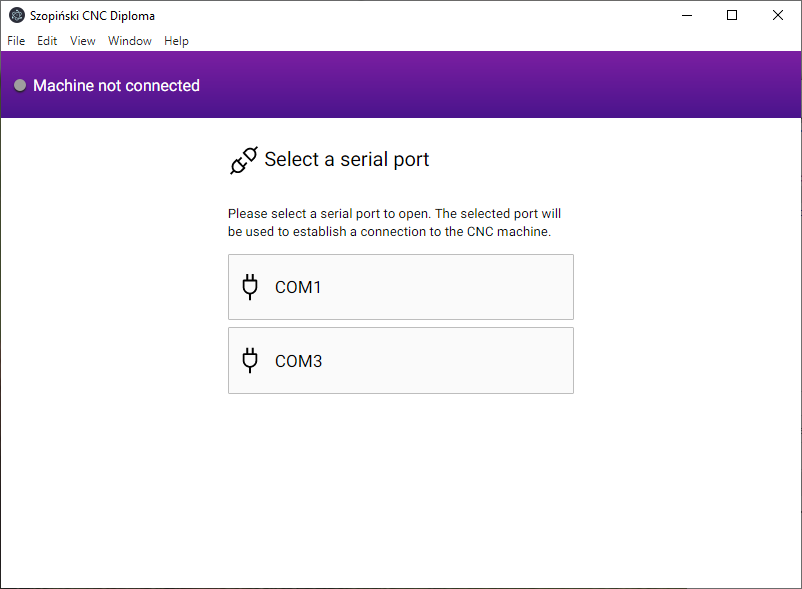
\includegraphics[width=0.75\linewidth]{serialselect}
        \caption{Serial port selection screen of the control software}
        \label{serialselect}
    \end{center}
\end{figure}

The control software is implemented using Electron, a framework for writing
desktop applications using web technologies. This allows it to present an
elegant, modern user interface while retaining the ability to perform low-level
operations such as serial communication. It also makes it easy to achieve
cross-platform compatibility.

Electron applications are written in JavaScript. They consist of a main process,
which interacts with the operating system, and a renderer process, which
displays the user interface in a browser window and exchanges information with
the main process. This ensures security in case the renderer process becomes
compromised.

Web development practices favor the use of externally developed software to
solve commonly encountered problems. Such software is distributed in the form of
packages and installed by a package manager. Every project has a list of
dependencies which must be collected before it is run.

The following libraries and tools were used to create this application:

\begin{itemize}
    \item Yarn, a combined package manager and project manager. Used for
    managing dependencies and launching build utilities \cite{yarn}.
    \item Webpack, a module bundler. Needed to compile the project into a
    compact set of files suitable for consumption by Electron \cite{webpack}.
    \item React, a framework for building user interfaces. It introduces a
    system of components and a mechanism to coordinate the flow of information
    within the application \cite{react}.
    \item React Redux, a library for managing the global application state.
    Facilitates handling events which impact multiple unrelated parts of the
    user interface \cite{redux}.
    \item React Router, a library to handle screen navigation \cite{router}.
    \item Node SerialPort, a JavaScript wrapper around the operating system's
    serial interface \cite{nodeserial}.
    \item Sass, a dialect of CSS which introduces a hierarchical structure
    \cite{sass}.
    \item ESLint, a code analysis tool for detecting errors and enforcing code
    style \cite{eslint}.
\end{itemize}

Because the application does not fetch data from the Internet nor does it
execute code from the file system, the renderer process is allowed to interact
with the operating system directly. This simplifies program design by removing
the need to communicate with the main process. The main process is thus reduced
to boilerplate code which opens the browser window and loads an HTML document
containing the application.

\subsubsection{Global program state}

\begin{figure}[ht]
    \begin{center}
        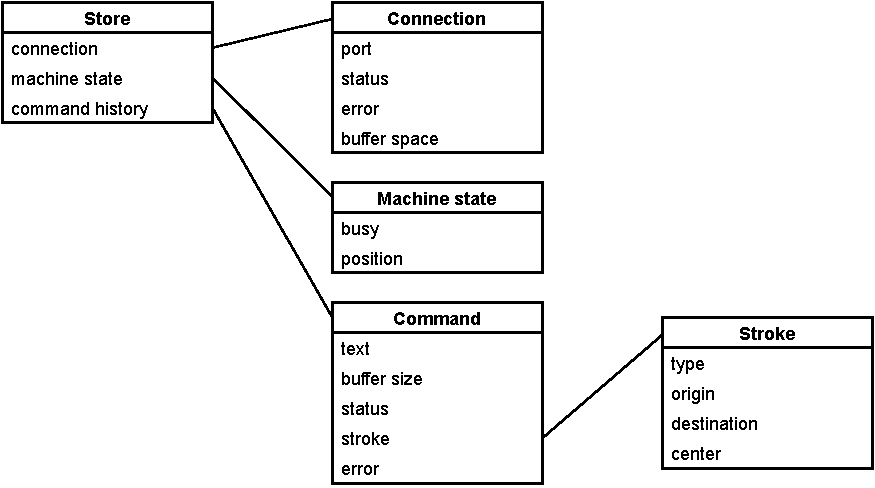
\includegraphics[width=0.75\linewidth]{globalstate}
        \caption{Structure of the store}
        \label{store}
    \end{center}
\end{figure}

Main program functionality is centered around the global state object, which
by Redux terminology is referred to as the \textit{store}. Redux introduces the
following design principles \cite{redux}:
\begin{enumerate}
    \item The store may only be changed by dispatching \textit{actions}, which
    may be thought of as events. Actions are dispatched in response to user
    interaction or incoming or outgoing serial traffic. Actions are handled
    by \textit{reducer} functions, which dictate how they impact the store.
    \item Changes in the store may be \textit{subscribed to} by various
    components of the program. When subscribers detect that a relevant part
    of the store has changed, they may trigger appropriate behavior.
\end{enumerate}

The store is divided into three top-level objects (figure~\ref{store}):
connection state, machine state, and command history. Changes to the connection
state cause the program to establish or to close a serial connection. The
machine state object reflects feedback received from the device, and is observed
by the user interface. The command history object governs data transmission
to the device and allows the user to monitor the execution of commands.

\subsubsection{Serial communication}

\begin{figure}[ht]
    \begin{center}
        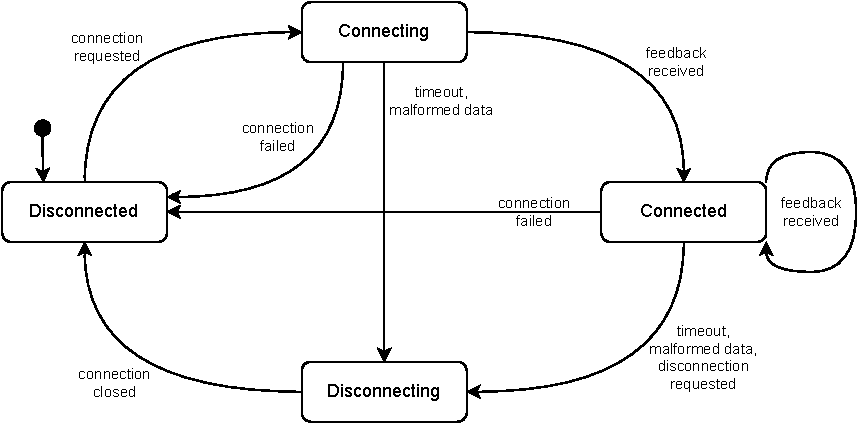
\includegraphics[width=0.75\linewidth]{serialstate}
        \caption{State transition of the serial connection}
        \label{serialstate}
    \end{center}
\end{figure}

A global store subscriber is registered to handle serial communication. When the
user first launches the application, they are presented with a serial port
selection screen (figure~\ref{serialselect}). Choosing one of the options
changes the connection status to \texttt{connecting}. The subscriber detects
this change and attempts to establish a new serial connection.

The device sends several kinds of feedback. The software verifies that the
feedback is received within a certain time frame and that it isn't malformed.
Violating the serial protocol terminates the connection. Receiving valid
feedback marks the connection as established (see figure~\ref{serialstate}).

There are three types of feedback packets:

\begin{itemize}
    \item Position feedback, sent every quarter second. Receiving this packet
    updates the store's machine state and establishes the connection.
    \item ``Command started'' feedback, sent once a command has been executed
    but before its motion has finished. Contains an interpretation of the
    command by the machine's G-code parser. Receiving this packet updates
    the command history and triggers an attempt to send commands to the device
    (see next section).
    \item ``Command finished'' feedback, sent once the motion initiated by a
    command has finished or if there was no motion. Updates the command history.
\end{itemize}

\subsubsection{Command history and queue}
\label{sending}

\begin{figure}[ht]
    \begin{center}
        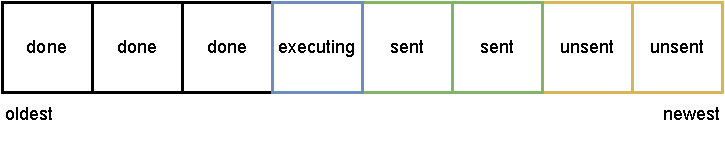
\includegraphics[width=0.6\linewidth]{commandhistory}
        \caption{Lifecycle of commands within the command history}
        \label{commandhistory}
    \end{center}
\end{figure}

In order to maintain a logical connection between sent commands and received
feedback, the application maintains a global command history object to
coordinate the exchange of data between the software and the firmware
(see figure~\ref{commandhistory}).

A command begins its lifecycle when a \texttt{sendCommand} action is dispatched.
The new command, whose status is \texttt{unsent}, is placed at the end of the
command history. The serial communication subscriber observes the history and
attempts to send the command, provided there are no other sent commands.

The device's receive buffer is limited in size and cannot handle an overflow
condition. For this reason, the software keeps track of the amount of available
buffer space and delays the transmission of commands as necessary. If the
command's content, encoded as UTF-8, is within this limit, the command is sent.
Its status is set to \texttt{sent} and its size is subtracted from the
available buffer space.

Once sent, the command is read and executed by the machine. When feedback
arrives, the command is marked as \texttt{executing}, its interpretation and
error code are updated, and its size is added back to the buffer space.
This prompts an attempt to send more commands.

Finally, once the command has been executed, its status is set to \texttt{done}.
Executed commands are purged from the history when no longer relevant to the
user.

\clearpage
\begin{figure}[ht]
    \begin{center}
        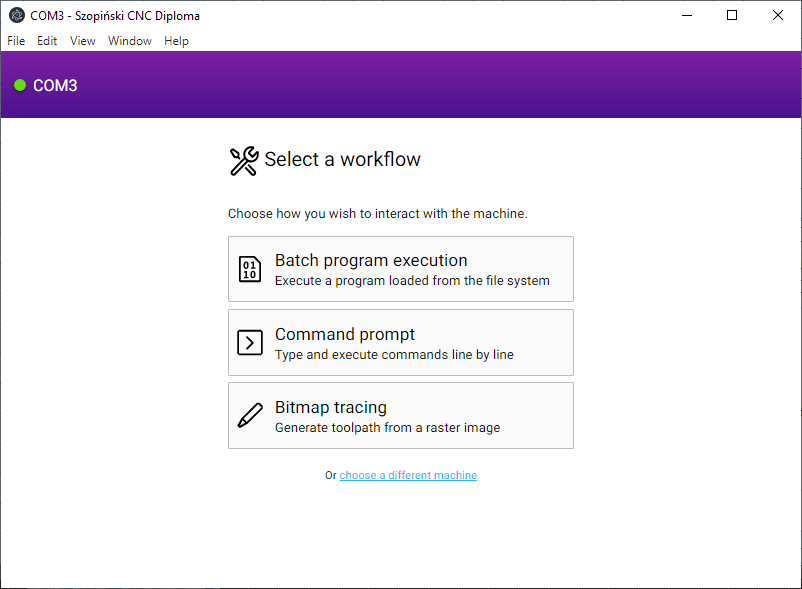
\includegraphics[width=0.8\linewidth]{workflowselect}
        \caption{Workflow selection screen}
        \label{workflow}
    \end{center}
\end{figure}
\begin{figure}[ht!]
    \begin{center}
        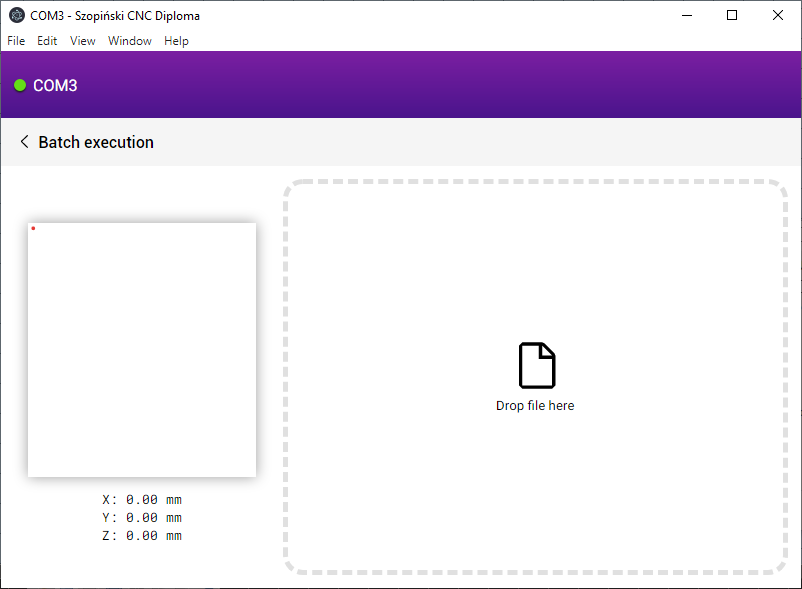
\includegraphics[width=0.8\linewidth]{batch}
        \caption{Batch execution screen, before dropping a file}
    \end{center}
\end{figure}

\clearpage
\begin{figure}[ht]
    \begin{center}
        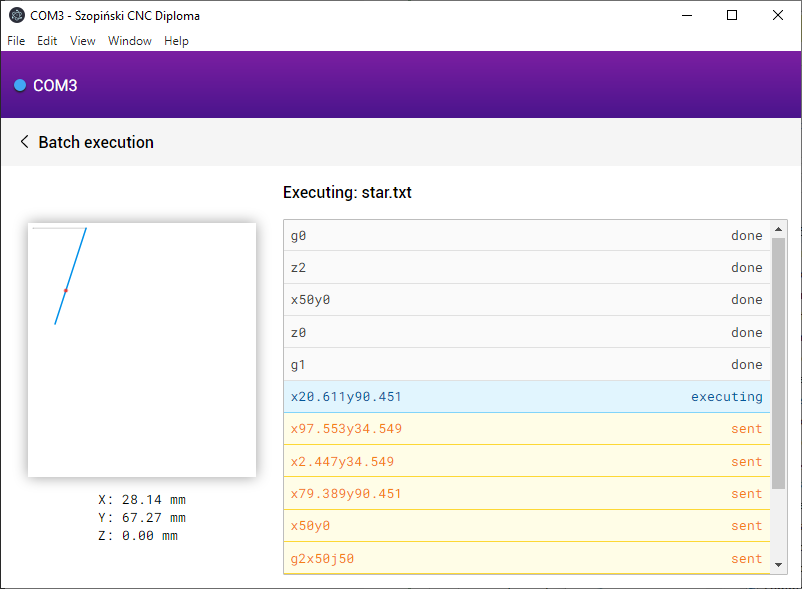
\includegraphics[width=0.8\linewidth]{batchexecuting}
        \caption{Batch execution screen, during execution}
        \label{batch}
    \end{center}
\end{figure}
\begin{figure}[ht!]
    \begin{center}
        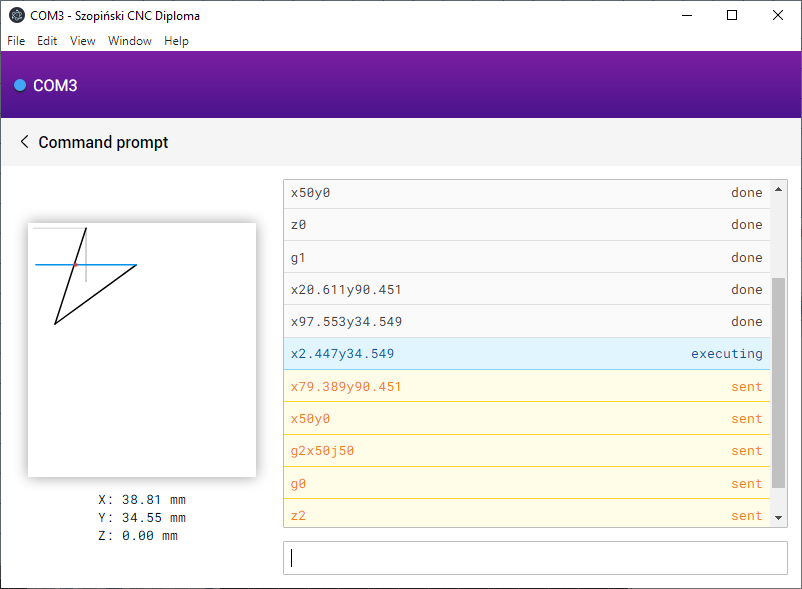
\includegraphics[width=0.8\linewidth]{commandprompt}
        \caption{Command prompt screen}
        \label{commandprompt}
    \end{center}
\end{figure}

\clearpage
\subsubsection{Motion preview}

When the application is launched, the user is presented with a workflow
selection screen (figure~\ref{workflow}). They may choose from three different
workflows: batch execution, command prompt and bitmap tracing. The first two
screens are simple interfaces exposing the functionality described in
section~\ref{sending}.

In each screen, the user may view a list of executing commands and a preview
of the motion initiated by them (figures~\ref{batch} and~\ref{commandprompt}).
The preview is generated by translating motion interpretation objects
(received as feedback from the machine) into SVG tags embedded directly in the
HTML document.

Translating linear motion is trivial. The SVG \texttt{line} element takes
arguments specifying an origin and a destination, which are given directly.
Rapid motion requires additional calculations for checking if it should be
split into two lines (as depicted in figure~\ref{rapid}). Translating circular
motion, however, is more complicated.

\begin{figure}[ht]
    \begin{center}
        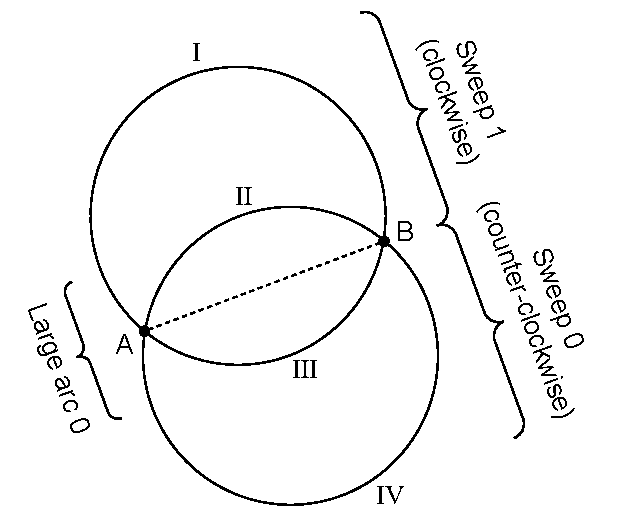
\includegraphics[width=0.4\linewidth]{arcflag}
        \caption{Four ways to draw an arc given two points and a radius}
        \label{arcflag}
    \end{center}
\end{figure}

In SVG, there are two ways to describe arcs. Full arcs may be drawn using the
\texttt{circle} element, which takes a radius and a center point. Partial
arcs can only be drawn with the \texttt{path} element and its \texttt{A}
instruction \cite{circles}. Because there are multiple paths through which two
points may be connected by an arc (figure~\ref{arcflag}), the \texttt{A}
instruction takes several arguments:

\begin{itemize}
    \item Implicit arc origin, $x_{orig}$ and $y_{orig}$
    \item $x$-axis radius $R_x$ and $y$-axis radius $R_y$
    \item $x$-axis rotation $\theta$
    \item Large arc flag $f_L$
    \item Sweep flag $f_S$
    \item Arc end, $x_{dest}$ and $y_{dest}$
\end{itemize}

The translation starts by calculating the radius. For circular arcs, the
$x$-axis radius and the $y$-axis radius are equal:
\begin{equation*}
    R_x = R_y = \sqrt{(x_{dest} - x_{center})^2 + (y_{dest} - y_{center})^2}
\end{equation*}
If the origin and the destination are the same, a \texttt{circle} element is
rendered and the calculation ends. Otherwise, the remaining arc parameters are
computed.

$x$-axis rotation $\theta$ is irrelevant for circles, therefore it is always
assigned a value of $0$. The sweep flag $f_S$ is conceptually equivalent to
drawing the arc in a clockwise or a counter\-clockwise manner, and so its value
is inferred from the motion type.
\begin{align*}
    \theta = 0 &&
    f_S = \begin{cases}
        1 & \text{for clockwise arcs} \\
        0 & \text{for counter-clockwise arcs}
    \end{cases}
\end{align*}

The large arc flag $f_L$ may be calculated by converting the origin and
destination points to polar coordinates relative to the arc center and measuring
the angular distance $\Delta$. If $\Delta$ exceeds $180\degree$, the arc is
large (figure~\ref{arctravel}).
\begin{gather*}
    \alpha = \text{atan2}(y_{orig} - y_{center}, x_{orig} - x_{center}) \\
    \beta = \text{atan2}(y_{dest} - y_{center}, x_{dest} - x_{center})
\end{gather*}
\begin{align*}
    \begin{aligned}
        \Delta_{cw} = \begin{cases}
            \beta - \alpha & \text{if } \alpha < \beta \\
            2\pi - \alpha + \beta & \text{otherwise}
        \end{cases} \\
        \Delta_{ccw} = \begin{cases}
            2\pi - \beta + \alpha & \text{if } \alpha < \beta \\
            \alpha - \beta & \text{otherwise}
        \end{cases}
    \end{aligned}
    &&
    f_L = \begin{cases}
        1 & \text{if } \Delta > \pi \\
        0 & \text{otherwise}
    \end{cases}
\end{align*}

\begin{figure}[ht]
    \begin{center}
        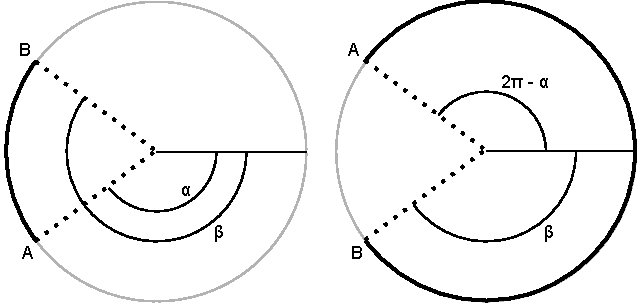
\includegraphics[width=0.6\linewidth]{arctravel}
        \caption{Measuring angular distance for clockwise arcs}
        \label{arctravel}
    \end{center}
\end{figure}

\clearpage
\subsubsection{Bitmap tracing}

\begin{figure}[ht]
    \begin{center}
        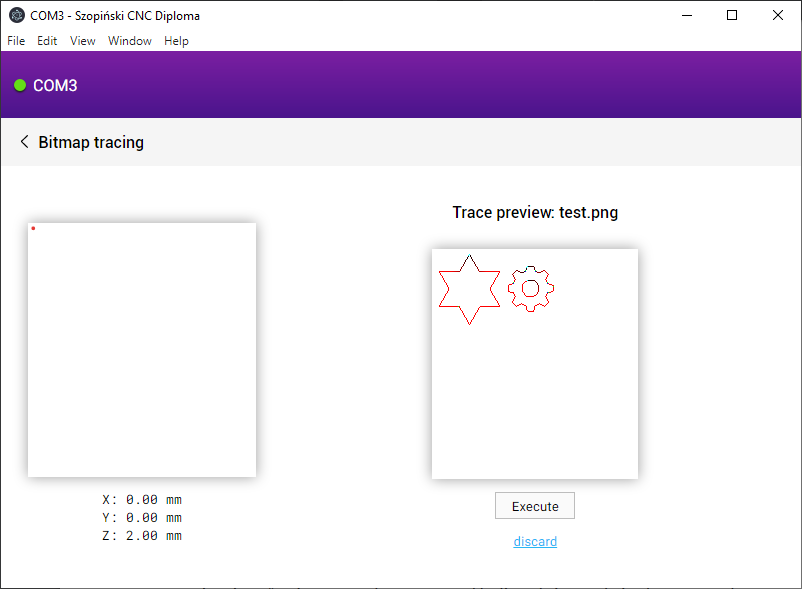
\includegraphics[width=0.75\linewidth]{trace}
        \caption{Bitmap tracing screen}
        \label{trace}
    \end{center}
\end{figure}

A major feature which makes the software user-friendly is bitmap tracing,
which takes a raster image and converts it to a sequence of G-code commands.
After the user uploads an image, they are presented with a preview of the
generated toolpath. They may execute the generated commands or discard the
result (figure~\ref{trace}).

Raster images contain no information about the curves they depict, however, a
vector approximation of an image may be constructed by linearly interpolating
between each marked pixel. A continuous sequence of points that may be drawn
without raising the tool is referred to as a \textit{segment}. Bitmap tracing
is implemented in five steps:
\begin{enumerate}
    \item Bitmap normalization, where the bitmap is reduced to a basic form
    \item Segment discovery, where continuous sequences of points are found
    \item Segment extension, where neighboring segments are connected
    \item Linear reduction, where unnecessary segment points are removed
    \item G-code generation, where segments are translated into commands
\end{enumerate}

Tracing begins by normalizing the input bitmap's dimensions and pixel data. The
bitmap is expanded to match the work area's aspect ratio. Transparency is
removed by superimposing the bitmap over a white background. Colors are
quantized such that if no channel R, G or B exceeds the value 127, a pixel
is made black, otherwise it is made white (figure~\ref{normalize}).

\clearpage
\begin{figure}[ht]
    \centering
    \begin{minipage}{0.5\textwidth}
        \centering
        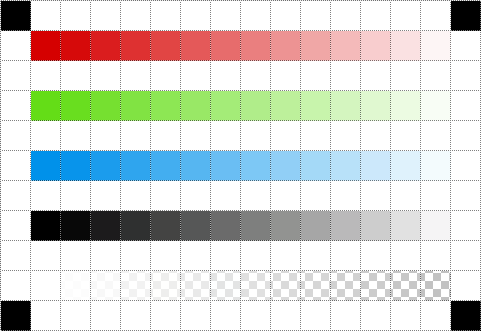
\includegraphics[width=0.5\textwidth]{normaltestin}
        \caption{Image before normalization}
    \end{minipage}\hfill
    \begin{minipage}{0.5\textwidth}
        \centering
        
\includegraphics[width=0.5\textwidth]{normaltestout}
        \caption{Image after normalization}
        \label{normalize}
    \end{minipage}
\end{figure}

Once the bitmap has been normalized, segment discovery begins. The bitmap is
scanned left-to-right, top-to-bottom in search of unexplored black pixels.
When such a pixel is encountered, it becomes the starting point of a new
segment. The program then attempts to include as many points in the segment as
possible, given certain constraints (figure~\ref{segments}).

\begin{figure}[ht]
    \begin{center}
        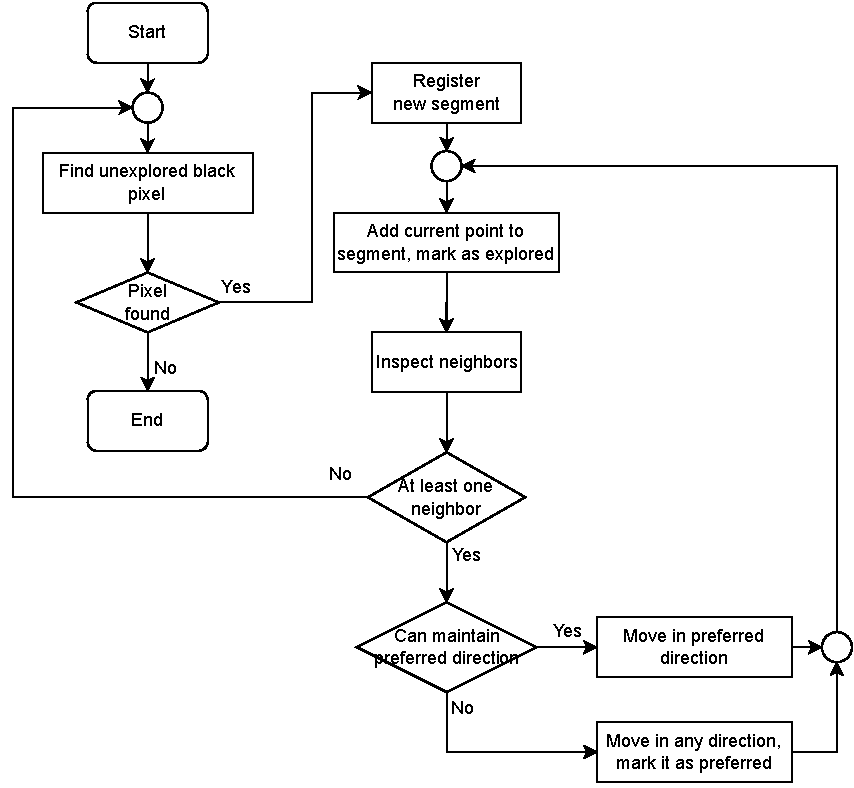
\includegraphics[width=0.6\linewidth]{segments}
        \caption{Flowchart of segment discovery and exploration}
        \label{segments}
    \end{center}
\end{figure}

On every iteration of the segment exploration algorithm, neighbors of the most
recently added pixel are inspected. If there are no neighbors eligible for
inclusion in the segment, the segment is terminated and the algorithm returns
to the scanning phase. This ensures that all pixels are eventually included in
a segment.

If there are multiple neighbors eligible for inclusion in a segment, the
algorithm gives preference to the one which maintains the current direction of
travel (figure~\ref{straight}). This reduces the amount of generated commands
by allowing multiple points to be covered by a single line.

\begin{figure}[ht]
    \begin{center}
        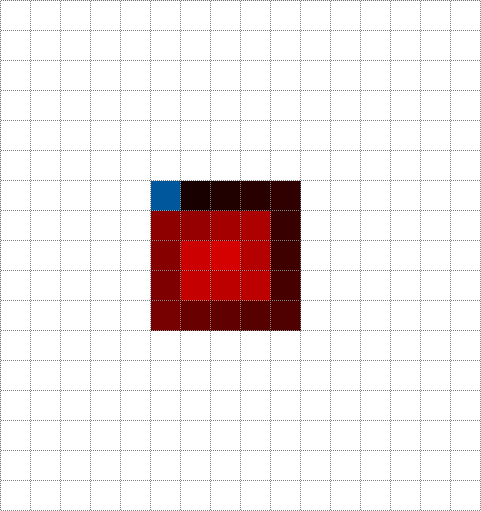
\includegraphics[width=0.25\linewidth]{straightpreview}
        \caption{Trace preview of a solid black square. Blue denotes segment
        origin, black-to-red gradient denotes segment progression}
        \label{straight}
    \end{center}
\end{figure}


Segments constructed in the described manner contain interpolations between
their constituent points, but not between other segments. To enable the
construction of more complex shapes, segments that neighbor other segments are
extended to maintain continuity. Segments whose terminal points neighbor each
other are extended to form loops.

Before segments are translated to G-code, an optimization is performed where
linear sequences are reduced to their terminal points. For each point of each
segment, if the following holds:
\begin{align*}
    \big(x - x_{prev} = x_{next} - x\big)
    \land
    \big(y - y_{prev} = y_{next} - y\big)
\end{align*}
then the point is eliminated.

Finally, G-code commands are generated from each segment. The machine makes a
rapid move to the initial point of a segment, lowers the tool, and then linearly
moves from one point to another. Once all segments have been drawn, the machine
returns to the coordinate origin.
